
%(BEGIN_QUESTION)
% Copyright 2007, Tony R. Kuphaldt, released under the Creative Commons Attribution License (v 1.0)
% This means you may do almost anything with this work of mine, so long as you give me proper credit

Twisted-pair Ethernet networks with more than two nodes must use some form of {\it hub} to connect everything together.  Each hub has a limited number of ports, but hubs may be cascaded to form networks larger than the port limit:

$$\includegraphics[width=15.5cm]{i02206x01.eps}$$

All hubs are not created equal, though -- they come in two varieties: {\it repeaters} and {\it switches}.  If we were to use simple {\it repeater} hubs, all five Ethernet DTE devices would belong to the same collision domain.  If we were to replace the middle repeater with a {\it switching} hub, however, we would have multiple collision domains instead of just one:

$$\includegraphics[width=15.5cm]{i02206x02.eps}$$

Explain how the operation of a switching hub (or just ``switch'') differs from a regular repeating hub, and how this difference results in the splitting of collision domains.

\underbar{file i02206}
%(END_QUESTION)





%(BEGIN_ANSWER)

A switch does not blindly broadcast all incoming data to all outgoing ports.  Instead, it learns what MAC address(es) reside on each port, and directs data frames only to their intended destination ports.

%(END_ANSWER)





%(BEGIN_NOTES)


%INDEX% Networking, Ethernet: collision domain
%INDEX% Networking, Ethernet: hub versus switch
%INDEX% Networking, Ethernet: switch versus hub

%(END_NOTES)


